\section{Thiết kế mạch khuếch đại dùng opamp tạo sóng ngõ ra và kiểm tra lại bằng proteus}	
		\subsection{Câu a.$\mathbf{v_o = 0.5 \cdot v_1 - 3 \cdot v_2 + 4 \cdot v_3}$}
			\subsubsection{Tính toán mạch khuếch đại dùng opamp}
				\begin{figure}[H]
					\centering
					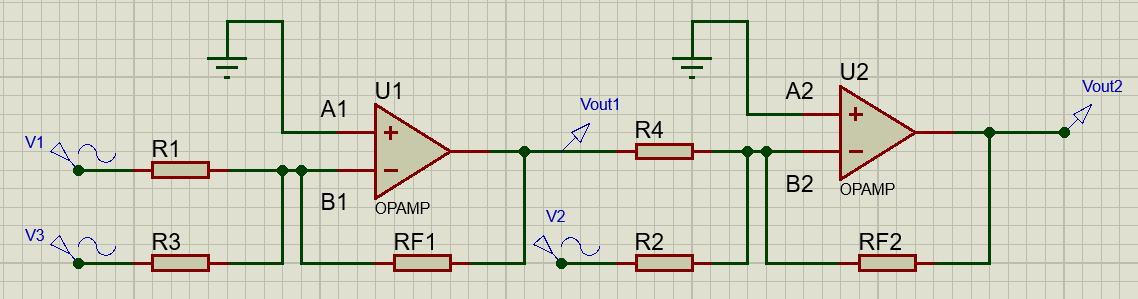
\includegraphics[width=0.7\textwidth]{pictures/topic1_a.png}
					\caption{Mạch khuếch đại dùng opamp}					
					\label{fig:circuit_simulation}
				\end{figure}
				\hspace*{0.6cm}\textbf{Giả sử KĐTT là lý tưởng}
				\[
				\Rightarrow
				\begin{cases}
					I^+ = I^- = 0\\
					V_{A1} = V_{B1} = V_{A2} = V_{B2} = 0\\
				\end{cases}
				\]
				\hspace*{0.6cm}Dòng điện đầu ra Opamp thứ nhất là:
				\begin{align}
					V_{out1} = -\frac{R_{F1}}{R_1} \cdot V_1 - \frac{R_{F1}}{R_3} \cdot V_3 
				\end{align}
				\hspace*{0.6cm}Dòng điện đầu ra Opamp thứ hai là:
				\begin{align}
					V_{out2} = -\frac{R_{F2}}{R_4} \cdot V_{out1} - \frac{R_{F2}}{R_2} \cdot V_2
				\end{align}
				\hspace*{0.6cm}Thế (1) vào (2) ta được: 
				\begin{align*}
					V_{out2} &= -\frac{R_{F2}}{R_4} \cdot \left(-\frac{R_{F1}}{R_1} \cdot V_1 - \frac{R_{F1}}{R_3} \cdot V_3\right) - \frac{R_{F2}}{R_2} \cdot V_2 \\
							&= \frac{R_{F1} \cdot R_{F2}}{R_1 \cdot R_4} \cdot V_1 + \frac{R_{F1} \cdot R_{F2}}{R_3 \cdot R_4} \cdot V_3 - \frac{R_{F2}}{R_2} \cdot V_2
				\end{align*}
				\hspace*{0.6cm}Theo đề bài ta có: $V_{out2} = 0.5 \cdot V_1 - 3 \cdot V_2 + 4 \cdot V_3$
				\[
				\Rightarrow
				\begin{cases}
					\frac{R_{F1} \cdot R_{F2}}{R_1 \cdot R_4} = 0.5\\
					\frac{R_{F1} \cdot R_{F2}}{R_3 \cdot R_4} = 4\\
					\frac{R_{F2}}{R_2} = 3
				\end{cases}
				\]
				\hspace*{0.6cm}Chọn $R_{2} = 50k\Omega$ $\Rightarrow$ $R_{F2} = 150k\Omega$.\\
				\hspace*{0.6cm}Chọn $R_{1} = 200k\Omega$, $R_{4} = 150k\Omega$ $\Rightarrow$ $R_{F1} = 100k\Omega$ $\Rightarrow$ $R_3 = 25k\Omega$.\\
			\newpage
			\subsubsection{Kiểm tra lại bằng proteus}
				\begin{itemize}
					\item Sử dụng Proteus để mô phỏng mạch như hình \ref{fig:circuit_simulation}
					\item Sử dụng các linh kiện: Opamp, Resistor, Voltage Source Sine, Ground
					\item Gán các giá trị điện trở như giá trị tính được ở trên.
					\item Cho các giá trị điện áp đầu vào $V_1 = 1V$, $V_2 = 2V$, $V_3 = 3V$.
					\item Kết quả mô phỏng được như hình \ref{fig:result_simulation}
					\begin{figure}[H]
						\centering
						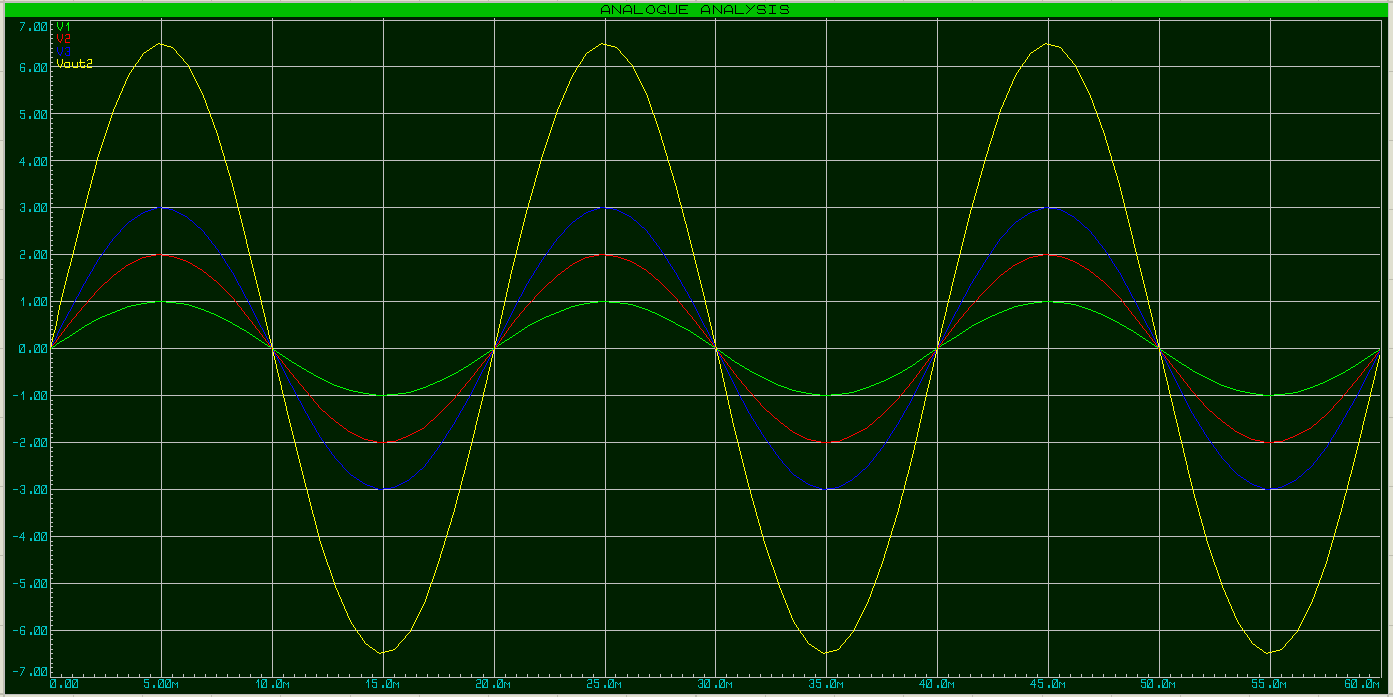
\includegraphics[width=0.7\textwidth]{pictures/result1_a.png}
						\caption{Mạch khuếch đại dùng opamp}					
						\label{fig:result_simulation}
					\end{figure}
					\item Ta thấy giá trị điện áp đầu ra $V_{out} = 0.5V_1 - 3V_2 + 4V_3 = 0.5 \cdot 1 - 3 \cdot 2 + 4 \cdot 3 = 6.5V$ giống với đồ thị analog $\Rightarrow$ Kết quả mô phỏng proteus giống với giá trị tính toán.
				\end{itemize}
		\subsection{Câu b.$\mathbf{v_o = 0.5 \cdot v_1(t) + 3 \int v_2(t)dt + 4\frac{dv_3(t)}{dt}}$}
			\subsubsection{Tính toán mạch khuếch đại dùng opamp}
				\begin{figure}[H]
					\centering
					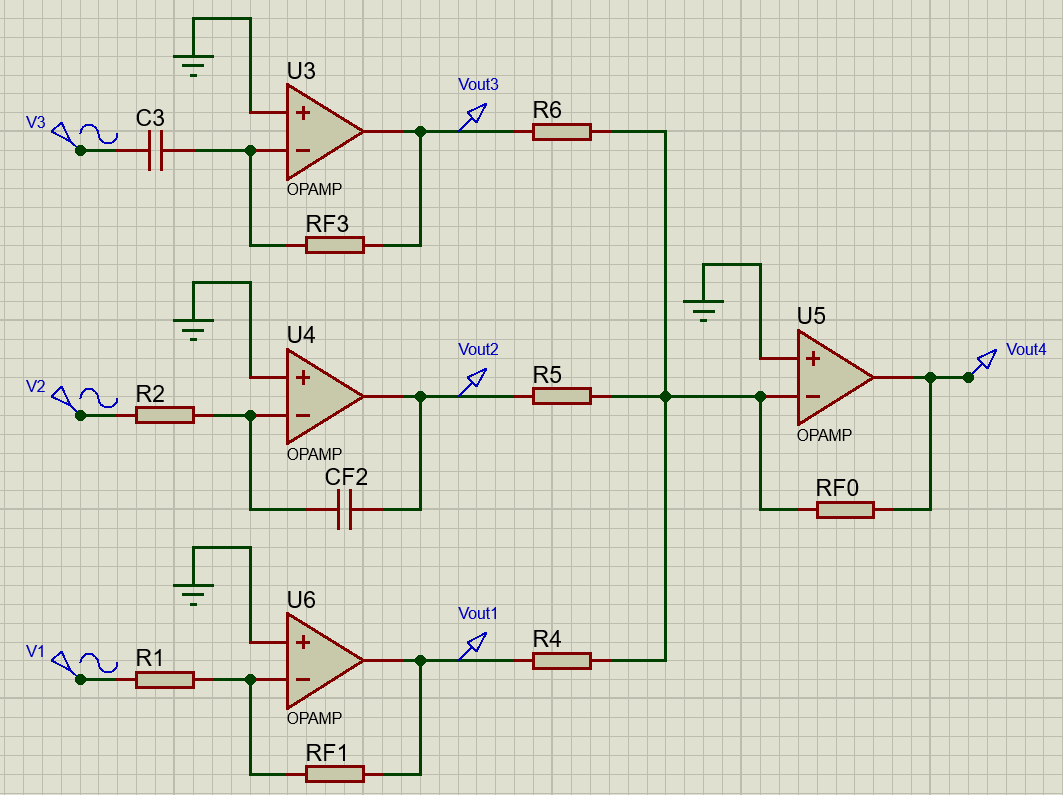
\includegraphics[width=0.7\textwidth]{pictures/topic1_b.png}
					\caption{Mạch khuếch đại dùng opamp}					
					\label{fig:circuit_simulation}
				\end{figure}
				\hspace*{0.6cm}\textbf{Giả sử KĐTT là lý tưởng}
				\[
				\Rightarrow
				\begin{cases}
					I^+ = I^- = 0\\
					V_{A1} = V_{B1} = V_{A2} = V_{B2} = 0\\
				\end{cases}
				\]
				\hspace*{0.6cm}Dòng điện đầu ra Opamp thứ nhất là:
				\begin{align}
					V_{out1} = -\frac{R_{F1}}{R_1} \cdot V_1
				\end{align}
				\hspace*{0.6cm}Dòng điện đầu ra Opamp thứ hai là:
				\begin{align}
					V_{out2} = -\frac{1}{R_2 \cdot C_{F2}} \cdot \int V_{2} dt
				\end{align}
				\hspace*{0.6cm}Dòng điên đầu ra Opamp thứ ba là:
				\begin{align}
					V_{out3} = -R_{F3} \cdot C_{3} \cdot \frac{dV_{3}(t)}{dt}
				\end{align}
				\hspace*{0.6cm}Dòng điện đầu ra Opamp thứ tư là:
				\begin{align}
					V_{out4} = -\frac{R_{F0}}{R_4} \cdot V_{out1} - \frac{R_{F0}}{R_5} \cdot V_{out2} - \frac{R_{F0}}{R_6} \cdot V_{out3}
				\end{align}
				\hspace*{0.6cm}Thế (3), (4), (5) vào (6) ta được:
				\begin{align*}
					V_{out4} &= -\frac{R_{F0}}{R_4}\left(-\frac{R_{F1}}{R_1} \cdot V_1\right) - \frac{R_{F0}}{R_5}\left(-\frac{1}{R_2 \cdot C_{F2}} \cdot \int V_{2} dt\right) - \frac{R_{F0}}{R_6}\left(-R_{F3} \cdot C_{3} \cdot \frac{dV_{3}(t)}{dt}\right)\\
						 &= \frac{R_{F1} \cdot R_{F0}}{R_1 \cdot R_4} \cdot V_1 + \frac{R_{F0}}{R_2 \cdot R_5 \cdot C_{F2}} \cdot \int V_{2} dt + \frac{R_{F0} \cdot R_{F3} \cdot C_{3}}{R_6} \cdot \frac{dV_{3}(t)}{dt}
				\end{align*}
				\newpage
				Theo đề bài ta có: $V_{out4} = 0.5 \cdot V_1 + 3 \int V_{2} dt + 4 \frac{dV_{3}(t)}{dt}$ 
				\[
				\Rightarrow
				\begin{cases}
					\frac{R_{F1} \cdot R_{F0}}{R_1 \cdot R_4} = 0.5\\
					\frac{R_{F0}}{R_2 \cdot R_5 \cdot C_{F2}} = 3\\
					\frac{R_{F0} \cdot R_{F3} \cdot C_{3}}{R_6} = 4
				\end{cases}
				\]
				\hspace*{0.6cm}Chọn $R_{1} = R_{F1} = R_{4} = 120k\Omega$ $\Rightarrow$ $R_{F0} = 60k\Omega$.\\
				\hspace*{0.6cm}Chọn $R_{2} = R_{5} = 100k\Omega \Rightarrow C_{F2} = 2\mu F$\\
				\hspace*{0.6cm}Chọn $R_{6} = 30k\Omega, R_{F3} = 200k\Omega \Rightarrow C_{3} = 10\mu F$.\\
			\subsubsection{Kiểm tra lại bằng proteus}
				\begin{itemize}
					\item Sử dụng Proteus để mô phỏng mạch như hình \ref{fig:circuit_simulation}
					\item Sử dụng các linh kiện: Opamp, Resistor, Capacitor, Voltage Source Sine, Ground
					\item Gán các giá trị điện trở và tụ như giá trị tính được ở trên.
					\item Cho các giá trị điện áp đầu vào $V_1 = 1V$, $V_2 = 2V$, $V_3 = 3V$.
				\end{itemize}
		
		